\documentclass[11pt]{beamer}\usepackage[]{graphicx}\usepackage[]{xcolor}
% maxwidth is the original width if it is less than linewidth
% otherwise use linewidth (to make sure the graphics do not exceed the margin)
\makeatletter
\def\maxwidth{ %
  \ifdim\Gin@nat@width>\linewidth
    \linewidth
  \else
    \Gin@nat@width
  \fi
}
\makeatother

\definecolor{fgcolor}{rgb}{0.345, 0.345, 0.345}
\newcommand{\hlnum}[1]{\textcolor[rgb]{0.686,0.059,0.569}{#1}}%
\newcommand{\hlstr}[1]{\textcolor[rgb]{0.192,0.494,0.8}{#1}}%
\newcommand{\hlcom}[1]{\textcolor[rgb]{0.678,0.584,0.686}{\textit{#1}}}%
\newcommand{\hlopt}[1]{\textcolor[rgb]{0,0,0}{#1}}%
\newcommand{\hlstd}[1]{\textcolor[rgb]{0.345,0.345,0.345}{#1}}%
\newcommand{\hlkwa}[1]{\textcolor[rgb]{0.161,0.373,0.58}{\textbf{#1}}}%
\newcommand{\hlkwb}[1]{\textcolor[rgb]{0.69,0.353,0.396}{#1}}%
\newcommand{\hlkwc}[1]{\textcolor[rgb]{0.333,0.667,0.333}{#1}}%
\newcommand{\hlkwd}[1]{\textcolor[rgb]{0.737,0.353,0.396}{\textbf{#1}}}%
\let\hlipl\hlkwb

\usepackage{framed}
\makeatletter
\newenvironment{kframe}{%
 \def\at@end@of@kframe{}%
 \ifinner\ifhmode%
  \def\at@end@of@kframe{\end{minipage}}%
  \begin{minipage}{\columnwidth}%
 \fi\fi%
 \def\FrameCommand##1{\hskip\@totalleftmargin \hskip-\fboxsep
 \colorbox{shadecolor}{##1}\hskip-\fboxsep
     % There is no \\@totalrightmargin, so:
     \hskip-\linewidth \hskip-\@totalleftmargin \hskip\columnwidth}%
 \MakeFramed {\advance\hsize-\width
   \@totalleftmargin\z@ \linewidth\hsize
   \@setminipage}}%
 {\par\unskip\endMakeFramed%
 \at@end@of@kframe}
\makeatother

\definecolor{shadecolor}{rgb}{.97, .97, .97}
\definecolor{messagecolor}{rgb}{0, 0, 0}
\definecolor{warningcolor}{rgb}{1, 0, 1}
\definecolor{errorcolor}{rgb}{1, 0, 0}
\newenvironment{knitrout}{}{} % an empty environment to be redefined in TeX

\usepackage{alltt}

%\usetheme{metropolis}
\usetheme[progressbar=head]{metropolis}
\defaultfontfeatures{ Scale = MatchUppercase }
\defaultfontfeatures[\rmfamily]{ Scale = 1}
\usepackage{unicode-math}

\usepackage{fontspec}
%\setmainfont[Scale = 0.95]{Lucida Bright OT}
%\setsansfont[Scale = 0.95]{Lucida Sans OT}
%\setmonofont[Scale = 0.80]{Lucida Console DK}

%\newfontfamily\meteoconsfont{Meteocons}
%\newcommand\meteocons[1]{{\meteoconsfont\symbol{#1}}}
%\newcommand\meteosun{\meteocons{"0042}}
%\newcommand\meteosuncloud{\meteocons{"0048}}
%\newcommand\meteorain{\meteocons{"0052}}
%\newcommand\meteosolidsun{\meteocons{"0031}}

\newfontfamily\lineabasicfont{linea-basic-10}
\newcommand\basicicons[1]{{\lineabasicfont\symbol{#1}}}
\newcommand\timeforwards{\basicicons{"0079}}
\newcommand\timebackwards{\basicicons{"0064}}

\newfontfamily\lineaweatherfont{linea-weather-10}
\newcommand\weathericons[1]{{\lineaweatherfont\symbol{#1}}}
\newcommand\meteosun{\weathericons{"E038}}
\newcommand\meteosuncloud{\weathericons{"E042}}
\newcommand\meteorain{\weathericons{"E033}}
\newcommand\meteowind{\weathericons{"E054}}

\newfontfamily\uleaffont{Mini Pics Uprooted Leaf}
\newcommand\uleafmpics[1]{{\uleaffont\symbol{#1}}}
\newcommand\lowplants{\uleafmpics{"00CE}}
\newcommand\mediumplant{\uleafmpics{"006A}}
\newcommand\bush{\uleafmpics{"0039}}
\newcommand\smallplant{\uleafmpics{"0030}}

\newfontfamily\KRfarmfont{KR Back On The Farm}
\newcommand\KRfarm[1]{{\KRfarmfont\symbol{#1}}}
\newcommand\farmplant{\KRfarm{"0049}}

\usepackage{framed}

\usepackage{tikz}
\usetikzlibrary{positioning,fit,arrows}

\tikzset{
 a/.style
  = {node distance=4em, text width=2.7em, minimum height=4em},
 b/.style
  = {rectangle, draw, fill=gray!10, node distance=4em, text width=6em,
     text centered, rounded corners, minimum height=4em, thick},
 c/.style
  = {circle, draw, dashed, fill=orange!10, inner sep = 0pt, node distance=5em, thick},
 d/.style
  = {rectangle, draw, dashed, fill=red!10, node distance=4em, text width=6em,
     text centered, rounded corners, minimum height=4em, thick},
 l/.style
  = {draw, -latex, thick},
 lr/.style
  = {draw, latex-latex, thick, red},
 lb/.style
  = {draw, -latex, thick, blue},
  lo/.style
  = {draw, -latex, thick, orange},
  lg/.style
  = {draw, -latex, thick, green},
  mylabel/.style
  ={text width=6.5em, text centered}
}

\usepackage{abbrev}

%\usepackage[style=authoryear-comp,firstinits,sortcites,maxcitenames=2,%
%    mincitenames=1,maxbibnames=10,minbibnames=10,uniquename=mininit,%
%    uniquelist=minyear,sortfirstinits=true]{biblatex}
%\usepackage[backend=biber,style=alphabetic]{biblatex}
\usepackage[style=authoryear-comp,firstinits,sortcites,maxcitenames=2,%
    mincitenames=1,maxbibnames=10,minbibnames=10,uniquename=mininit,%
    uniquelist=minyear,sortfirstinits=true]{biblatex}
\addbibresource{info4plants.bib}
%\renewcommand{\bibfont}{\small}
\IfFileExists{upquote.sty}{\usepackage{upquote}}{}
\begin{document}





\pgfdeclareimage[height=10ex]{SenPEP_large}{figures/senpep_logo}
\pgfdeclareimage[width=0.19\textwidth]{SenPEP}{figures/senpep_logo}
\pgfdeclareimage[width=0.19\textwidth]{HYflame}{figures/HY_biot_text}
\pgfdeclareimage[width=0.15\textwidth]{ViPS}{figures/senpep_logo}
\pgfdeclareimage[width=0.12\textwidth]{SMS}{figures/SMS}
\pgfdeclareimage[width=0.11\textwidth]{ESP}{figures/ESP}
\pgfdeclareimage[width=0.15\textwidth]{ViPS}{figures/vips-logo}
\pgfdeclareimage[width=0.15\textwidth]{AKA}{figures/aka_logo}

\title{The evolutionary ecology of information acquisition in plants}
\subtitle{The basis of brainless forecasting}
\author{Pedro J. Aphalo}
\date{Camp Evolution VII, 2 March 2020}
\institute[Univ.\ of Helsinki]{Organismal and Evolutionary Biology Research Programme\\[1ex] and\\[1ex] Viikki Plant Science Center, University of Helsinki\\[1ex] \href{http://blogs.helsinki.fi/senpep-blog/}{\pgfuseimage{SenPEP_large}} }


	\begin{frame}
		\maketitle
	\end{frame}


%	\begin{frame}
%		\frametitle{Outline}
%		\tableofcontents
%	\end{frame}

\section{Background}

\begin{frame}
\frametitle{Warning}
\begin{itemize}
  \item Much of my talk is based on reshuffling my ideas together with Ariel's\ldots
  \item \ldots combined with some fundamental insights I gained here from Alex's talks.
  \item Main one being, that much of what we heard from Alex about control systems and evolution, is applicable also to acclimation.
  \item Here I will not attempt to describe evolution as a control system\ldots
  \item \ldots but rather think of light perception as the input boundary of a physiological/developmental control system.
\end{itemize}
\end{frame}

\begin{frame}
  \frametitle{Acclimation depends on plasticity}
\begin{itemize}
  \item Responses take time $\Rightarrow$ must be triggered in advance.
  \item Slow responses need to be triggered earlier than fast ones.
  \item Enhanced readiness to respond allows delaying full commitment.
  \item Prediction of future environment is error-prone.
  \item Cost of response is deterministic, benefit is stochastic.
  \item Acclimation is based on syndromes rather than individual responses (?).
\end{itemize}
\end{frame}

\begin{frame}
\frametitle{Sunlight}
\begin{knitrout}\scriptsize
\definecolor{shadecolor}{rgb}{0.969, 0.969, 0.969}\color{fgcolor}

{\centering \includegraphics[width=.95\textwidth]{figure/pos-plant-vision-00-1} 

}


\end{knitrout}
\end{frame}

\begin{frame}
\frametitle{Perception of daylight by humans vision}
\begin{itemize}
\item Wavelengths from 380 to 720 nm are visible.
\item Three photoreceptors $\rightarrow$ 1 million colours.
\item The photoreceptors are sensitive to red (R), green (G) and blue photos (B).
\item Colour sensation is the result of information processing\ldots
\item \ldots which maps the excitation of the three photoreceptors into ``expected'' colours.
\item i.e., colour TV, film photogarphy, digital photography, most colour printing, mixing to pigments by artist, all target human vision.
\end{itemize}
\end{frame}

\begin{frame}
\frametitle{Human (cone fundamentals)}
\begin{knitrout}\scriptsize
\definecolor{shadecolor}{rgb}{0.969, 0.969, 0.969}\color{fgcolor}\begin{kframe}


{\ttfamily\noindent\bfseries\color{errorcolor}{\#\# Error in spct\_class \%in\% photobiology::spct\_classes(): argument "{}spct\_class"{} is missing, with no default}}\end{kframe}
\end{knitrout}
\end{frame}

\begin{frame}
\frametitle{Perception of daylight by plants}
\begin{itemize}
\item Wavelengths from $\approx 270$\,nm to $\approx 800$ are perceptible.
\item About 14 photoreceptors $\rightarrow$ RGB, far-red (FR) and ultraviolet (UV); only 5 colours (??!!).
\item Some photoreceptors have different modes of action leading to different sets of responses.
\item Photoreceptors can function as wavelength-ratio detectors, as flux detectors or time-domain-integrators.
\end{itemize}
\end{frame}

\begin{frame}
\frametitle{Plants (phytochromes)}
\begin{knitrout}\scriptsize
\definecolor{shadecolor}{rgb}{0.969, 0.969, 0.969}\color{fgcolor}

{\centering \includegraphics[width=.95\textwidth]{figure/pos-plant-vision-0-1} 

}


\end{knitrout}
\end{frame}

\begin{frame}
\frametitle{Plants (cryptochromes)}
\begin{knitrout}\scriptsize
\definecolor{shadecolor}{rgb}{0.969, 0.969, 0.969}\color{fgcolor}\begin{kframe}


{\ttfamily\noindent\color{warningcolor}{\#\# Warning in normalize\_spct(spct = T2A(x, action = "{}replace"{}), range = range, : Normalization not updated: unsupported old object)}}

{\ttfamily\noindent\color{warningcolor}{\#\# Warning in normalize\_spct(spct = T2A(x, action = "{}replace"{}), range = range, : Normalization not updated: unsupported old object)}}\end{kframe}

{\centering \includegraphics[width=.95\textwidth]{figure/pos-plant-vision-1-1} 

}


\end{knitrout}
\end{frame}

\begin{frame}
\frametitle{Plants (phototropins)}
\begin{knitrout}\scriptsize
\definecolor{shadecolor}{rgb}{0.969, 0.969, 0.969}\color{fgcolor}\begin{kframe}


{\ttfamily\noindent\color{warningcolor}{\#\# Warning in normalize\_spct(spct = T2A(x, action = "{}replace"{}), range = range, : Normalization not updated: unsupported old object)}}

{\ttfamily\noindent\color{warningcolor}{\#\# Warning in normalize\_spct(spct = T2A(x, action = "{}replace"{}), range = range, : Normalization not updated: unsupported old object)}}\end{kframe}

{\centering \includegraphics[width=.95\textwidth]{figure/pos-plant-vision-2-1} 

}


\end{knitrout}
\end{frame}

\begin{frame}
\frametitle{Plants (UVR8)}
\begin{knitrout}\scriptsize
\definecolor{shadecolor}{rgb}{0.969, 0.969, 0.969}\color{fgcolor}\begin{kframe}


{\ttfamily\noindent\color{warningcolor}{\#\# Warning in normalize\_spct(spct = T2A(x, action = "{}replace"{}), range = range, : Normalization not updated: unsupported old object)}}\end{kframe}

{\centering \includegraphics[width=.95\textwidth]{figure/pos-plant-vision-3-1} 

}


\end{knitrout}
\end{frame}

\begin{frame}
\frametitle{Plants (UVR8 $\times$ sunlight)}
\begin{knitrout}\scriptsize
\definecolor{shadecolor}{rgb}{0.969, 0.969, 0.969}\color{fgcolor}\begin{kframe}


{\ttfamily\noindent\color{warningcolor}{\#\# Warning in normalize\_spct(spct = e2q(x, action = "{}replace.raw"{}), range = range, : Normalization not updated: unsupported old object)}}\end{kframe}

{\centering \includegraphics[width=.95\textwidth]{figure/pos-plant-vision-4-1} 

}


\end{knitrout}
\end{frame}


\begin{frame}%[<+->]
  \frametitle{Vocabulary: information as an abstraction}
  \begin{itemize}
    \item Information is encoded in one or more carrier.
    \item e.g.\ radio broadcasting vs.\ internet-``radio''.
    \item First a signal (or cue) needs to be sensed or perceived.
    \item To extract information a signal or cue must be decoded.
    \item The components of a signal or cue that we cannot decode into information we call ``noise''.
    \item Memory is the storage of information.
    \item Processing is the combination of different bits of information.
    \item Communication is the exchange of information (between an emitter and a receiver, can be one-way or two way).
  \end{itemize}
\end{frame}

\begin{frame}%[<+->]
  \frametitle{Forecasting: its relation to fitness}
  \begin{itemize}
\item Our everyday life depends on forecasting all sorts of events every minute.
    \item Sometimes we do this consciously, but most of the time we are not aware of what our brain is doing.
    \item Perception of cues and memories are sources of information.
    \item e.g.\ estimating the weight of a cup when lifting it.
  \end{itemize}
\end{frame}

\begin{frame}%[<+->]
  \frametitle{Forecasting: its relation to fitness}
  \begin{itemize}
    \item I ask you to forget about how its processing is implemented\ldots
    \item \ldots and consider the idea that every organism must have evolved the capacity to ``forecast'' future events important for its fitness.
    \item How information is processed, ``the machinery used'', does not need to be the same as long the information is acquired, transmitted, stored and combined successfully.
  \end{itemize}
\end{frame}

\begin{frame}%[<+->]
\frametitle{Information as a paradigm}
\begin{enumerate}
  \item Information and big data are the buzz-words or our time.
  \item Given us a paradigm that ``asks to be applied''\ldots
  \item \ldots but care is needed.
  \item Much like the machine paradigm from the industrial revolution failed to explain life\ldots
  \item \ldots the use-of-information paradigm will not be enough to explain it.
  \item However, it is able to explain some aspects of life.
\end{enumerate}
\end{frame}

\begin{frame}%[<+->]
\frametitle{Forecasting for economic investment}
\begin{enumerate}
  \item There are reliable and unreliable sources of information.
  \item Forecasting can depend on a single reliable predictor or\ldots
  \item \ldots on a combination of several less reliable predictors.
  \item Predictors \emph{do not need} to have a direct cause-effect relationship.
  \item Forecasts are subject to errors\ldots
  \item \ldots with outcomes that can be described by probabilities.
  \item A dynamic context requires repeated-tuning of models.
\end{enumerate}
\end{frame}

\begin{frame}
  \frametitle{Correlations in the environment}
  \includegraphics[width=\linewidth]{figures/cor_examples2.pdf}
\end{frame}

\begin{frame}%[<+->]
\frametitle{Cues and signals as sources of information}
\begin{enumerate}
  \item Cue/signal and predicted event need to be correlated.
  \item Cross-correlation and autocorrelation both work.
  \item The sign of correlation is irrelevant.
  \item Cue/signal should precede the predicted event\ldots
  \item \ldots long enough for acclimation to take place.
  \item Correlation can be spatial, temporal or both.
  \item ``Random noise'' in spatial/temporal cues/signals can be ``smoothed out''.
\end{enumerate}
\end{frame}

\begin{frame}
\frametitle{Listener perspective}
\begin{enumerate}
  \item Contribution to own fitness
  \item Own response
  \item Decoding of information
  \item Perception
  \item Available cues/signals
\end{enumerate}
\end{frame}

\begin{frame}
\frametitle{Emitter perspective}
\begin{enumerate}
  \item Contribution to own fitness
  \item Response from listener
  \item Encoding of information
  \item Emission
  \item Broadcasted signals
\end{enumerate}
\end{frame}

\begin{frame}
\frametitle{Data processing mechanism in plants I}
\begin{itemize}
  \item We know something on how decoding works\ldots
  \item \ldots for some individual cues or signals.
  \item A frequent \emph{naive model} is a linear chain of events.
  \item Cue/signal perception $\rightarrow$ direct decoding of information $\rightarrow$ response
  \item Low R:FR $\rightarrow$ ``means shade'' $\rightarrow$ shade avoidance response
  \item Can frequently describe responses to single cues or signals
\end{itemize}
\end{frame}

\begin{frame}
\frametitle{Data processing mechanism in plants II}
\begin{itemize}
  \item We know almost nothing on how decoding works\ldots
  \item[] \ldots for sets of cues or signals.
  \item A complex and realistic (?) model is a network of interactions, memories and feedback loops.
  \item Synchronous and asynchronous perception of cues/signals $\rightarrow$ \ldots
  \item[] complex decoding of information (1) $\rightarrow$\ldots
    adjustment of ready-ness to respond.
  \item Synchronous and asynchronous perception of cues/signals $\rightarrow$ \ldots
  \item[] complex decoding of information + readiness state $\rightarrow$ response.
\end{itemize}
\end{frame}

\section{A possible framework}

\begin{frame}{Information-based framework for acclimation}

\begin{itemize}
\item<1-11>[]Conceptual framework\vspace{1ex}\pause

\centering
\resizebox{\linewidth}{!}{%
\tiny
  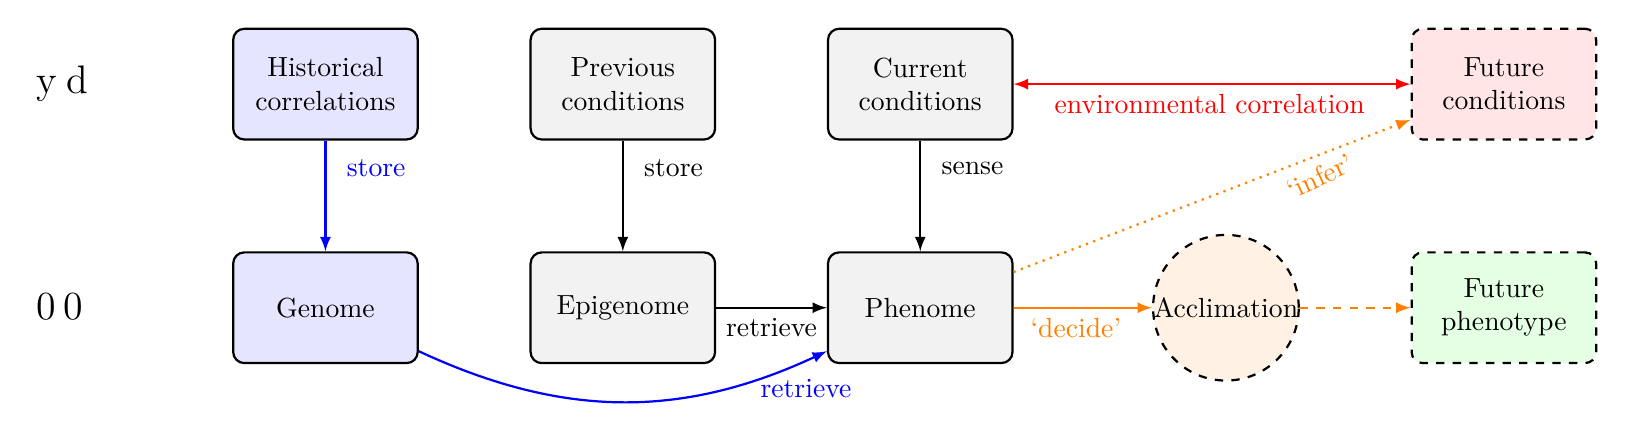
\begin{tikzpicture}[auto]
    \node [a] (environment) {\Large\timeforwards~\timebackwards};
    \node [b, right = of environment, fill=blue!10] (history) {Historical correlations};
    \node [b, right = of history] (stress) {Previous conditions};
    \node [b, right = of stress] (data) {Current conditions};\pause
    \node [b, below = of stress] (memory) {Epigenome};
    \node [b, right = of memory] (info) {Phenome};
    \node [b, below = of history, fill=blue!10] (genome) {Genome};
    \node [a, below = of environment] (plant) {\Large\smallplant\,\smallplant};\pause
    \node [c, right = of info, fill=orange!10] (acclimation) {Acclimation};
    \node [d, right = of acclimation, fill=green!10] (ready) {Future phenotype};
    \node [d, above = of ready] (stress2) {Future conditions};\pause

    \path [l] (stress) -- (memory) node[near start,right]{\hspace{0.4em}store};
    \path [lb] (history) -- (genome) node[near start, right]{\hspace{0.4em}store};\pause
    \path [l] (data) -- (info) node[near start,right]{\hspace{0.4em}sense};
    \path [l] (memory) -- (info) node[near start,below]{\hspace{2em}retrieve};
    \path [lb] (genome) edge [bend right=25]  node[near end, right]{\hspace{1em}retrieve} (info);\pause
    \path [lr] (stress2) -- (data) node[near end,below]{\hspace{7em}environmental correlation};\pause
    \path [lo, dotted] (info) -- (stress2) node[near end,below,rotate=25]{`infer'};\pause
    \path [lo] (info) -- (acclimation) node[near start,below]{\hspace{2em}`decide'};\pause
    \path [lo, dashed] (acclimation) -- (ready);

\end{tikzpicture}%
}%


\item<11>[]Example: Frost hardening\vspace{1ex}\pause

\centering
\resizebox{\linewidth}{!}{%
\tiny
  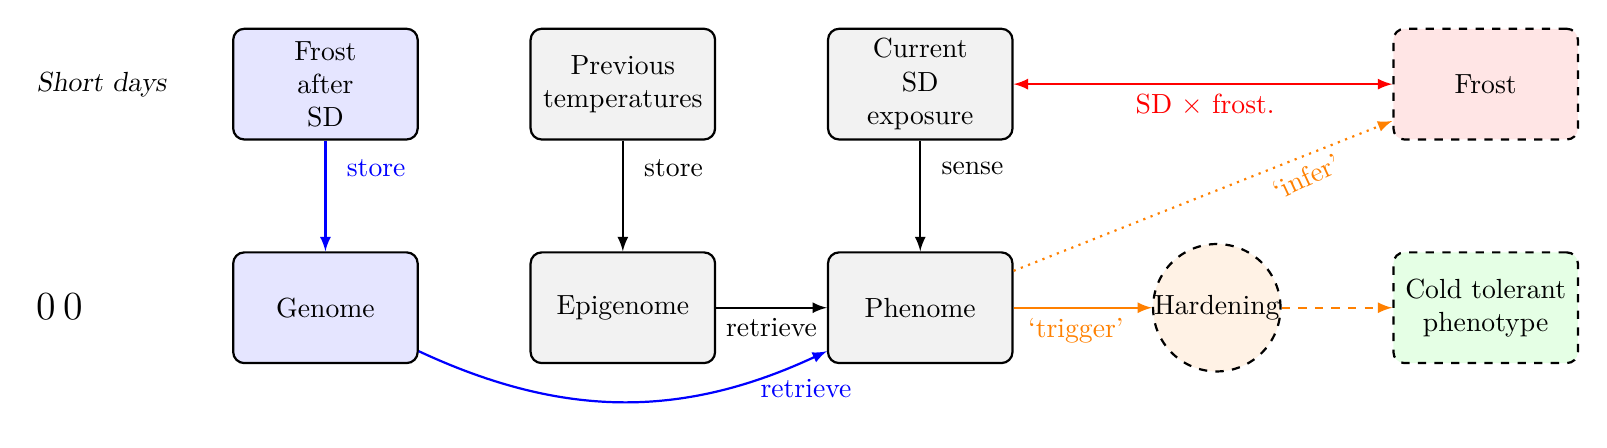
\begin{tikzpicture}[auto]
    \node [a] (environment) {\textsl{Short~days}};
    \node [b, right = of environment, fill=blue!10] (history) {Frost\\after\\SD};
    \node [b, right = of history] (stress) {Previous temperatures};
    \node [b, right = of stress] (data) {Current\\SD\\exposure};
    \node [b, below = of stress] (memory) {Epigenome};
    \node [b, right = of memory] (info) {Phenome};
    \node [b, below = of history, fill=blue!10] (genome) {Genome};
    \node [a, below = of environment] (plant) {\Large\smallplant\,\smallplant};
    \node [c, right = of info, fill=orange!10] (acclimation) {Hardening};
    \node [d, right = of acclimation, fill=green!10] (ready) {Cold tolerant phenotype};
    \node [d, above = of ready] (stress2) {Frost};

    \path [l] (stress) -- (memory) node[near start,right]{\hspace{0.4em}store};
    \path [lb] (history) -- (genome) node[near start, right]{\hspace{0.4em}store};
    \path [l] (data) -- (info) node[near start,right]{\hspace{0.4em}sense};
    \path [l] (memory) -- (info) node[near start,below]{\hspace{2em}retrieve};
    \path [lb] (genome) edge [bend right=25]  node[near end, right]{\hspace{1em}retrieve} (info);
    \path [lr] (stress2) -- (data) node[near end,below]{\hspace{7em}SD $\times$ frost.};
    \path [lo, dotted] (info) -- (stress2) node[near end,below,rotate=25]{`infer'};
    \path [lo] (info) -- (acclimation) node[near start,below]{\hspace{2em}`trigger'};
    \path [lo, dashed] (acclimation) -- (ready);

\end{tikzpicture}%
}

\end{itemize}
\end{frame}

\begin{frame}{Proposed theoretical framework (II)}

\begin{itemize}
\item<1-2>[]Conceptual framework\vspace{1ex}

\centering
\resizebox{\linewidth}{!}{%
\tiny
  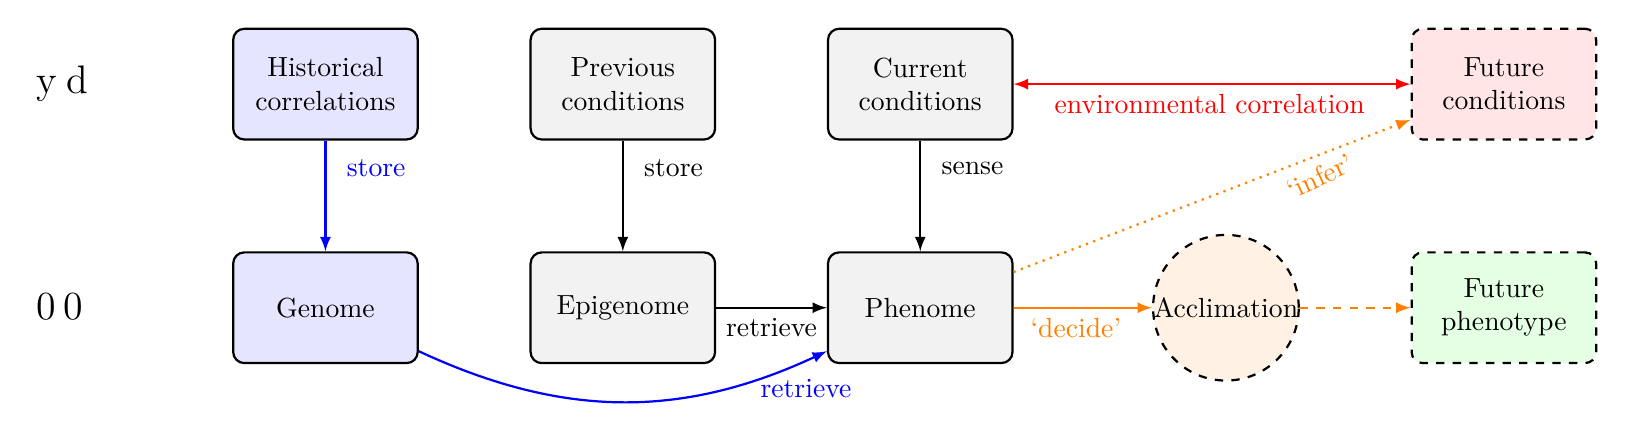
\begin{tikzpicture}[auto]
    \node [a] (environment) {\Large\timeforwards~\timebackwards};
    \node [b, right = of environment, fill=blue!10] (history) {Historical correlations};
    \node [b, right = of history] (stress) {Previous conditions};
    \node [b, right = of stress] (data) {Current conditions};
    \node [b, below = of stress] (memory) {Epigenome};
    \node [b, right = of memory] (info) {Phenome};
    \node [b, below = of history, fill=blue!10] (genome) {Genome};
    \node [a, below = of environment] (plant) {\Large\smallplant\,\smallplant};
    \node [c, right = of info, fill=orange!10] (acclimation) {Acclimation};
    \node [d, right = of acclimation, fill=green!10] (ready) {Future phenotype};
    \node [d, above = of ready] (stress2) {Future conditions};

    \path [l] (stress) -- (memory) node[near start,right]{\hspace{0.4em}store};
    \path [lb] (history) -- (genome) node[near start, right]{\hspace{0.4em}store};
    \path [l] (data) -- (info) node[near start,right]{\hspace{0.4em}sense};
    \path [l] (memory) -- (info) node[near start,below]{\hspace{2em}retrieve};
    \path [lb] (genome) edge [bend right=25]  node[near end, right]{\hspace{1em}retrieve} (info);
    \path [lr] (stress2) -- (data) node[near end,below]{\hspace{7em}environmental correlation};
    \path [lo, dotted] (info) -- (stress2) node[near end,below,rotate=25]{`infer'};
    \path [lo] (info) -- (acclimation) node[near start,below]{\hspace{2em}`decide'};
    \path [lo, dashed] (acclimation) -- (ready);

\end{tikzpicture}%
}%

\item<2>[]UVB example\vspace{1ex}

\centering
\resizebox{\linewidth}{!}{%
\tiny
  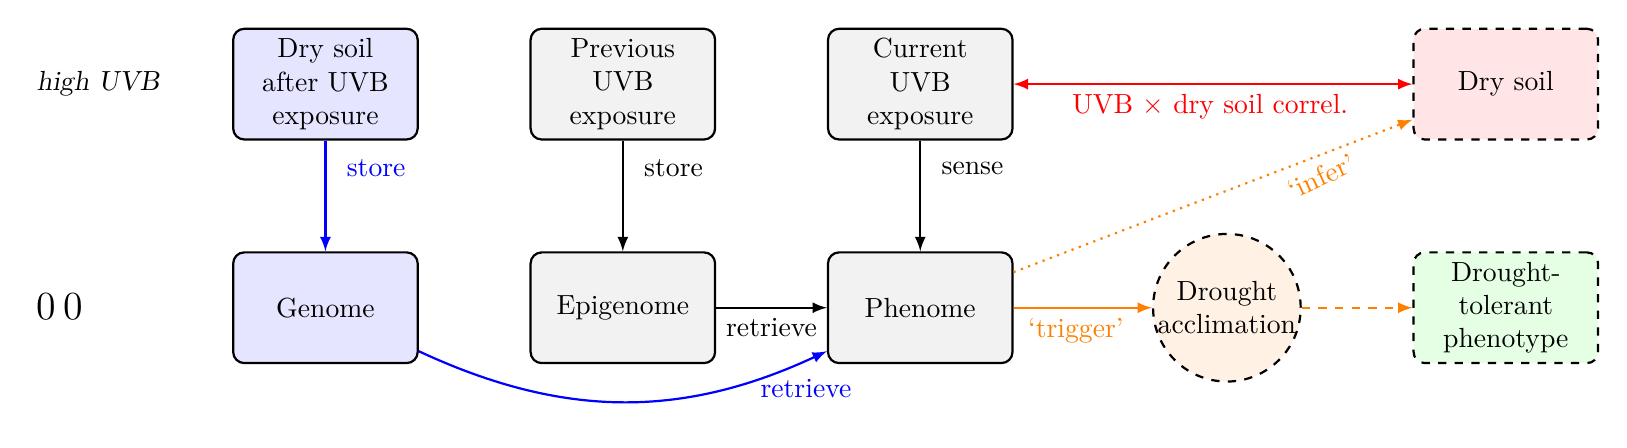
\begin{tikzpicture}[auto]
    \node [a] (environment) {\textsl{high~UVB}};
    \node [b, right = of environment, fill=blue!10] (history) {Dry soil\\ after UVB\\ exposure};
    \node [b, right = of history] (stress) {Previous\\ UVB\\ exposure};
    \node [b, right = of stress] (data) {Current\\ UVB\\ exposure};
    \node [b, below = of stress] (memory) {Epigenome};
    \node [b, right = of memory] (info) {Phenome};
    \node [b, below = of history, fill=blue!10] (genome) {Genome};
    \node [a, below = of environment] (plant) {\Large\smallplant\,\smallplant};
    \node [c, right = of info, fill=orange!10] (acclimation) {\parbox{5em}{\centering Drought\\ acclimation}};
    \node [d, right = of acclimation, fill=green!10] (ready) {Drought-tolerant phenotype};
    \node [d, above = of ready] (stress2) {Dry soil};

    \path [l] (stress) -- (memory) node[near start,right]{\hspace{0.4em}store};
    \path [lb] (history) -- (genome) node[near start, right]{\hspace{0.4em}store};
    \path [l] (data) -- (info) node[near start,right]{\hspace{0.4em}sense};
    \path [l] (memory) -- (info) node[near start,below]{\hspace{2em}retrieve};
    \path [lb] (genome) edge [bend right=25]  node[near end, right]{\hspace{1em}retrieve} (info);
    \path [lr] (stress2) -- (data) node[near end,below]{\hspace{7em}UVB $\times$ dry soil correl.};
    \path [lo, dotted] (info) -- (stress2) node[near end,below,rotate=25]{`infer'};
    \path [lo] (info) -- (acclimation) node[near start,below]{\hspace{2em}`trigger'};
    \path [lo, dashed] (acclimation) -- (ready);

\end{tikzpicture}%
}%
\end{itemize}
\end{frame}

\section{Implications}

\begin{frame}
  \frametitle{Context matters for signalling}
  \begin{enumerate}
    \item Components of signalling networks can be best teased out in unnatural contexts including single factor experiments.
    \item Regulation and signalling interactions can be meaningfully described only in real or realistic contexts preferably using factorial experiments.
    \item Real contexts are variable, so ample replication is needed.
    \item Describing a syndrome requires in most cases parallel measurements at different levels of organization.
    \item Time courses of response need to be followed.
  \end{enumerate}
\end{frame}

\begin{frame}
  \frametitle{Data analysis and interpretation}
  \begin{itemize}
    \item Search for patterns of response across mutants and treatments/conditions.
    \item Be careful about quality of gene annotations.
    \item Be very careful about gene ontology (GO) terms.
    \item With PCR have enough reference genes.
  \end{itemize}
\end{frame}

\end{document}

	\begin{frame}[c]
		\begin{center}
			\begin{small}
				\copyright 2016--2020 by Pedro J. Aphalo\\
				Organismal and Evolutionary Biology Research Programme, University of Helsinki, Finland.\\
				\textcolor{blue}{\url{http://blogs.helsinki.fi/senpep-blog/}}\\[2ex]
			\end{small}

			\begin{footnotesize}
				`The evolutionary ecology of information acquisition in plants' slides from a presentation by Pedro J. Aphalo are licensed under a Creative Commons Attribution-ShareAlike 4.0 International License.\\[2ex]

			\end{footnotesize}

			\includegraphics[width=6em]{figures/by-sa}
		\end{center}
	\end{frame}
